\documentclass[11pt]{article}

%%% Load some useful packages:
%% "New" LaTeX2e graphics support.
\usepackage{graphicx}
%%	using final option to force graphics to be included even in draft mode
%\usepackage[final]{graphicx}
\usepackage{paralist} % compact lists

%% Support sub-figures.
\usepackage{subfigure}

%% Make subsubsections numbered and included in ToC
\setcounter{secnumdepth}{3}
\setcounter{tocdepth}{3}

%% Package to linebreak URLs in a sane manner.
\usepackage{url}

%% Define a new 'smallurl' style for the package that will use a smaller font.
\makeatletter
\def\url@smallurlstyle{%
  \@ifundefined{selectfont}{\def\UrlFont{\sf}}{\def\UrlFont{\small\ttfamily}}}
\makeatother
%% Now actually use the newly defined style.
\urlstyle{smallurl}

%% Make margins less ridiculous
\usepackage{fullpage}

%% Allows insertion of fixme notes for future work
\usepackage[footnote, nomargin]{fixme}

%%%% Turned off for tech report, should be turned on for research portfolio
%% Turn on double spacing
%\usepackage{setspace}
%\doublespacing

%% Make URLs clickable
\usepackage[colorlinks, bookmarks=true]{hyperref}
\usepackage[all]{hypcap}


%% Since I'm using the LaTeX Makefile that uses dvips, I need this
%% package to make URLs break nicely
\usepackage{breakurl}

\usepackage{array}

%% Adds new functionality for tables
\usepackage{tabularx}

\newcolumntype{P}[1]{>{\raggedright\arraybackslash}p{#1}}

% create a shortcut to typeset table headings
\newcommand\tabhead[1]{\small\textbf{#1}}

\usepackage{multirow}

%% Make table cross pages.
\usepackage{longtable}

%% Provides customization of lists
\usepackage{enumitem}

%% Now define question list type
\newlist{question}{enumerate}{1}
\setlist[question]{resume, label=\textbf{\arabic*.}}

%% Define multiple choice answer list type
\newlist{answer}{enumerate}{1}
\setlist[answer]{label=\alph*)}

%% Provides some useful symbols such as checkboxes, circles
\usepackage{wasysym}

%% Define checkbox answer list type
\newlist{checkbox}{itemize}{1}
\setlist[checkbox]{label=\Square}

%% Define radio button answer list type
\newlist{radiobutton}{itemize}{1}
\setlist[radiobutton]{label=\Circle}


\begin{document}

\title{SGSEAM Assessment Plan for Makahiki}

\author{
	 Yongwen Xu \\
\em  Collaborative Software Development Laboratory \\
\em  Department of Information and Computer Sciences \\
\em  University of Hawai'i at Manoa\\
     yxu@hawaii.edu \\
}

\date{June 2013}
\maketitle

\tableofcontents

\graphicspath{{figures/}} 
\DeclareGraphicsExtensions{.eps}


\chapter{SGSEAM Plan for Makahiki }
\label{app:makahiki-assessment-plan}

This appendix includes the SGSEAM assessment plan for Makahiki. It is the deliverable for the first step of SGSEAM when applying to Makahiki framework. It first identifies the stakeholders, determines the appropriate assessment
approaches according to the available resources, chooses assessment participants, and creates the assessment schedule.

\section{Identify SGSEAM Stakeholders in Makahiki}
The first step in SGSEAM assessment plan is to identify the stakeholders in Makahiki. \autoref{table:eval-stakeholders} listed the identified stakeholders who use the Makahiki framework. 

\begin{table}[ht!]
  \centering
  \begin{tabular}{|p{0.2\columnwidth}|p{0.4\columnwidth}|p{0.3\columnwidth}|}
    \hline
    \tabhead{Stakeholder class} &
    \tabhead{Tasks} &
    \tabhead{Role} \\
    \hline
    Player &
    Participate in the Makahiki games &
    Students living in the residential halls\\
    \hline
    System admin &
    Install Makahiki software, monitor and scale the system, backup, patch maintenance &
    IT staffs\\
    \hline
    Game designer &
    Design the content, configure suitable games and mechanics &
    Challenge organizers\\
    \hline
    Game manager &
    Manage the game during the period of game play.&
    Challenge organizers\\
    \hline
    Developer &
    Develop customization, extend and enhance the game and framework. &
    Makahiki developers \\
    \hline
  \end{tabular}
  \caption{SGSEAM Stakeholders}
  \label{table:eval-stakeholders}
\end{table}

\section {Determine SGSEAM Approaches for Makahiki}

The second step in SGSEAM plan is to determine the assessment approach. As described in SGSEAM, approaches include both  {\em in-vivo} and {\em in-vitro} assessments. The  {\em in-vivo} approaches, such as pre-post test, in-game surveys and post-hoc interviews, assess the real world instance of the game. The {\em in-vitro} approaches use in-lab experiments in a simulated environment. Different assessment approaches will have different levels of rigor or validity. When applying SGSEAM in Makahiki, I used the real world Makahiki instances as the in-vivo approaches which includes pre-post effectiveness study for player assessment, post-hoc interview for game administrator and game designer. 

In addition to real world instances assessment, I also implemented the in-vitro assessment approach using in-lab experiments. In Spring 2013, Professor Philip Johnson at the Information and Computer Science Department of University of Hawaii used Makahiki to teach a course in serious game development. The students were seniors or graduate students majoring in computer science related fields. During the course, the students installed Makahiki, designed a serious game instance with Makahiki, and developed an enhancement to the Makahiki system.
The participation was voluntary. This is considered as an in-lab experiment since they are evaluating Makahiki in a class setting and using Makahiki in the development environments.

\autoref{table:eval-approaches} lists the SGSEAM approaches that are used to assess the strengths and weaknesses of Makahiki from different stakeholders' view.

\begin{table}[ht!]
  \centering
  \begin{tabular}{|p{0.17\columnwidth}|p{0.32\columnwidth}|p{0.42\columnwidth}|}
    \hline
    \tabhead{Stakeholder}&
    \tabhead{Assessment approaches} &
    \tabhead{Expected Outcomes} \\
    \hline
    \multirow{4}{*}{Player} & Pre-post effectiveness study &
    Determine effectiveness in energy literacy and resource usage reduction \\
    \cline{2-3}
      & Self-reported effectiveness survey &
	Determine self-reported effectiveness in behavior change and awareness\\
    \cline{2-3}
    & Self-reported usability survey &
	Identify problem areas in game interface\\
    \cline{2-3}
     & Engagement metrics &
	Determine the extent of engagement\\
    \hline
    \multirow{2}{*}{System admin} & Post-hoc admin interview &
    \multirow{2}{0.42\columnwidth}{Determine strengths and weaknesses in system install and maintenance}\\
    \cline{2-2}
    & In-lab system admin study & \\
    \hline
    \multirow{2}{*}{Game designer} & Post-hoc designer interview &
	\multirow{2}{0.42\columnwidth}{Determine strengths and weaknesses in facilitating the game design process} \\
	\cline{2-2}	
	& In-lab game design study & \\
    \hline
   Game manager & Post-hoc manager interview & 
	Determine strengths and weaknesses in managing the game \\
    \hline
    Developer & In-lab game development study & 
        Determine strengths and weaknesses in developing system enhancement \\
    \hline
  \end{tabular}
  \caption{SGSEAM approaches}
  \label{table:eval-approaches}
\end{table}

The following sections describe the assessment approaches in details. 

\subsection{Player Assessment Plan}

I plan to use the real-world Makahiki instances (UHM KC 2011, 2012, 2014) at the University of Hawaii at Manoa to study the player's experience with the Makahiki framework. There will be over 1000 eligible players for each of these instances. The players are first year college students living in four similar structured residence halls in close vicinity. There are smart electrical meters installed in these residence halls.

To assess the effectiveness of the framework for designing games that improve player literacy in sustainability, we will 
conduct two energy literacy surveys, one before the challenge (pre-game) and one after
the challenge (post-game). SurveyGizmo will be used to create the surveys which consists of the set of sustainability literacy and behavior questionnaires. The response from the two surveys will be analyzed to provide insight about the player's literacy and behavior change. 

To assess the effectiveness of the framework for designing games that produce positive change in sustainability
behaviors, we will record and analyze the energy consumption data before, during and after the
challenge.  Before the challenge, an energy usage baseline will be established. The energy consumption data will be examined to understand any usage pattern or reduction during and after the challenge.  We will also conduct an in-game self-reported behavior change survey. The survey will ask questions about player interests in sustainability prior to and after the game, as well as any perceived behavior changes when playing the game. The in-game survey questionnaires are described in \autoref{app:in-game-questionnaire}.

To assess the usability of the game produced by the Makahiki framework, we will conduct an in-game usability survey. The survey will ask questions about the players' experience with respect to the user interface of the game. The response from the survey will be analyzed to provide insight about the game usability. 

In addition to the surveys and energy data measurement, the following engagement metrics will be calculated based on the game and log data to assess the engagement level of the instance:

\begin{itemize}
\item Participation rate
\item Number of players per day
\item Play time per day
\item Submissions per day
\item Social interactions per day
\item Website errors per day
\end{itemize}

\subsection{System Admin Assessment Plan}

I plan to use two approaches to assess the system admin's experience: One is an in-lab experiment, the other is interviews with the system admin of a real world Makahiki instance.

I will conduct an in-lab experiment with the students in the ICS691 (a serious game development class in the Department of Computer Science at UHM) in Spring 2013.  The students will be tasked with installing the Makahiki system into their local computers as well as the cloud environment. In order to understand how much time it takes to install the Makahiki and what problems might be encountered, I designed a Google form which details the steps for installing Makahiki both locally and in the cloud. I will ask students to use this form to record the time they spent and the problems they encountered during each step.

\autoref{fig:developer-eval-form} illustrates a partial google form used for Makahiki system admin assessment. \autoref{app:googleform} includes the complete google form.
\begin{figure}[ht!]
   \centering
   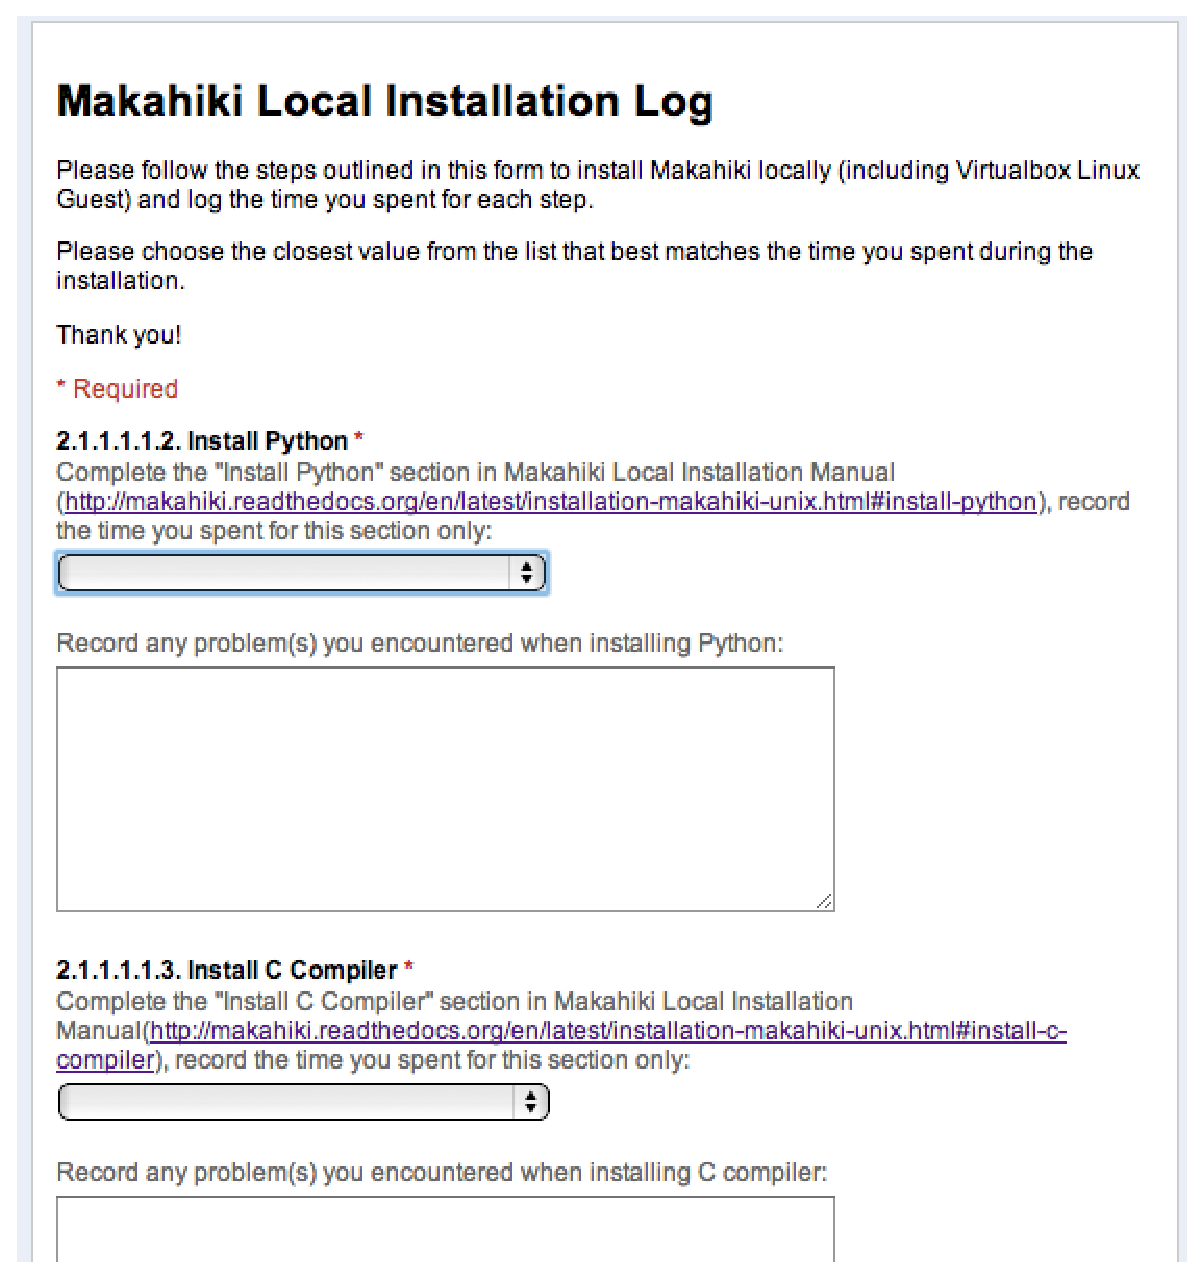
\includegraphics[height=30em,width=30em]{developer-eval-form.eps}
   \caption{Makahiki Developer assessment Form}
   \label{fig:developer-eval-form}
\end{figure}

The students will also be asked to provide feedback about their installation experiences in the form of a blog post. In the blog post, I will ask them to discuss the following topics:
\begin{itemize}
\item What is the most difficult step during installation?
\item What problems did you encounter during the installation?
\item Have you install any database, web server or similar server products prior to this assignment? Are those installations for development or production purpose?
\item If you have experience installing other servers before, How does your prior experience of installing other servers compare to the installation of Makahiki?
\item What could be improved about the Makahiki installation process?
\item Compare your experience of installing Makahiki in Heroku with installing it locally,
\end{itemize}

The data collected from the Google form responses and the blog posts from the students will be analyzed to gain insight into how easy or difficult it is to install Makahiki. 

In order to gain insight into the experience of a real world system admin who uses Makahiki, I will perform interviews to the system admin of the 2012 Hawaii Pacific University (HPU) challenge. The interview questions will include:
\begin{itemize}
 \item How much time did you spend to install the Makahiki system?
 \item How much time did you spend to maintain the Makahiki system, including backup, monitoring?
 \item What problems did you encounter during your installation and administering the Makahiki system?
\end{itemize}

I will also collect any email exchanges with the system admin regarding the installation process and maintenance of Makahiki system. Both interview and email exchange data will be analyzed to understand the system admin's experiences with Makahiki.  

\subsection{Game Designer Assessment Plan}

Similar to Makahiki system admin assessment, I plan to use two approaches to assess the game designer's experience: One is an in-lab experiment, the other is interviews with the game designers of real world Makahiki instances.

I will conduct an in-lab experiment with the same students in the ICS691 class. The students will be tasked to design a Kukui Cup-like serious game using Makahiki. I designed another Google form with the detailed steps for designing a game in Makahiki. I will ask students to follow these steps and record their time and problems encountered during their designing process. \autoref{app:googleform} has the complete Google form for the steps the students need to follow.

In addition, the students will be asked to provide feedback about their game design experiences in the form of blog posts that discuss the following topics:
\begin{itemize}
\item What is the most difficult step during Challenge Design?
\item What problems did you encounter while designing the challenge?
\item What could be improved in the Makahiki Challenge Design process?
\end{itemize}

The data collected from the responses of the game design Google forms and the blog posts from the students will be analyzed to gain insight into the game design experiences with Makahiki.

In order to gain insight into the experience of real world game designers who use Makahiki to design serious games, I will perform interviews with the real-world game designers of the 2012 Hawaii Pacific University challenge and the 2012 East West Center challenge. I will asked them about their experiences using the Makahiki game design admin interface to design their sustainability serious games. The interview questions will include:
\begin{itemize}
    \item How much time did you spend to configure the challenge global settings?
    \item How much time did you spend to design the individual games?
    \item What problems did you encounter?
    \item Did you find it difficult to design a specific game? which one, what was difficult?
    \item What did you like the least when using the system?
\end{itemize}

I will also collect any email exchanges with the game designers regarding the game design process. Both the interview and email exchange data will be analyzed to gain insight into the game design experiences with Makahiki.

\subsection{Game Manager Assessment Plan}

I plan to perform interviews with the real world game managers of the 2012 Hawaii Pacific University challenge and 2012 East West Center challenge to study the experience of game management using Makahiki. The interview questions will include:
\begin{itemize}
\item How much time did you spend to approve the action submissions?
\item How much time did you spend to monitor the game status?
\item What problems did you encounter?
\item Did you find it difficult to manage? what was difficult?
\item What did you like the least when using the system?
\end{itemize}

I will collect any email exchanges with the game managers. The data collected from the interviews and email exchanges will be analyzed to gain insight into the game managing experiences with Makahiki. 

\subsection{Developer Assessment Plan}

I plan to perform an in-lab game development study experiment with the students participating in the ICS691 serious game development class in Spring 2013. The students will be tasked with developing an enhancement to the Makahiki instance. This will involve setting up the development environment, following the tutorial to create the ``Hello world'' widget using Makahiki, and finally, developing an enhancement which extends the functionality of the Makahiki system. The enhancement is specified in 5 development tasks. 

The students will be asked to submit their development source code to the public source code repository (Github) and write a blog post to discuss their efforts in completing the development activities. The blog post should discuss the following topics:
\begin{itemize}
\item What part is complete?
\item What part is not complete?
\item Which parts you found easy or hard to complete?
\item What problems did you encounter while developing this enhancement tasks?
\item What is your recommendations for the framework to improve development support.
\end{itemize}

I will review their source code to compare their code to the reference implementation, analyze the blog posts, as well as any email correspondences regarding the problems encountered during the development. 

\section{Choose Assessment Participants}

After the assessment approaches are determined, the next step in SGSEAM is to identify the assessment participants for the different stakeholders. \autoref{table:sgseam-makahiki-participants} lists the participants for assessing the Makahiki framework using SGSEAM. 

\begin{table}[ht!]
  \centering
  \begin{tabular}{|p{0.2\columnwidth}|p{0.45\columnwidth}|p{0.2\columnwidth}|}
    \hline
    \tabhead{Stakeholder class} &
    \tabhead{Person(s)} &
    \tabhead{Organization} \\
    \hline
    Player &
    All eligible players in the UH KC instance &
    UHM \\
    \hline
    System admin &
    ICS691 students, \newline system admin for HPU instance &
    UHM, HPU\\
    \hline
    Game designer &
    ICS691 students, \newline game designers for HPU  \& EWC instance &
    UHM, HPU, EWC \\
    \hline
    Game manager &
    ICS691 students, \newline game managers for HPU \& EWC instance &
    UHM, HPU, EWC \\
    \hline
    Developer &
    ICS691 students &
    UHM\\
    \hline
  \end{tabular}
  \caption{SGSEAM Participants for Makahiki}
  \label{table:sgseam-makahiki-participants}
\end{table}

\section{Create Assessment Schedule}

After determining what the assessment approaches and who the participants are, the next step is to create the assessment 
schedule. The schedule for applying SGSEAM to Makahiki is shown in
\autoref{table:sgseam-makahiki-schedule}. 

\begin{table}[ht!]
  \centering
  \begin{tabular}{|p{0.18\columnwidth}|p{0.5\columnwidth}|p{0.18\columnwidth}|}
    \hline
    \tabhead{Time} &
    \tabhead{Task} &
    \tabhead{Assessment}  \\
    \hline
    Fall 2011 & Pre-post and in-game surveys, engagement metrics collection with UHM 2011 KC & Player experience\\
    \hline
    2012 & In-game survey, engagement metrics collection with UHM 2012 KC & Player experience\\
    \hline
    Fall 2012 & Interview with HPU KC sysadmin & System admin experience \\
    \hline
    Fall 2012 & Interview with HPU \& EWC KC game designers & Game designer experience \\
    \hline
    Fall 2012 & Interview with HPU \& EWC KC game managers & Game manager experience \\
    \hline
    Spring 2013 & In-lab installation experiment with UHM ICS691 students &  System admin experience \\
    \hline
    Spring 2013 & In-lab game design experiment with UHM ICS691 students & Game designer experience \\
    \hline
    Spring 2013 & In-lab game development experiment with UHM ICS691 students & Developer experience \\
    \hline
    Spring 2014 & in-game survey with UHM 2014 KC & Player experience \\
    \hline
  \end{tabular}
  \caption{SGSEAM Assessment Schedule for Makahiki}
  \label{table:sgseam-makahiki-schedule}
\end{table}


\appendix
\chapter{In-Game Survey Questionnaire}
\label{app:in-game-questionnaire}

This appendix details the contents of the questionnaire made available to participants via the in-game questionnaire during the UHM Makahiki challenge. Participants filled out the questionnaire via the SurveyGizmo~\cite{surveygizmo} website. The survey started with the informed consent via inputing  the email address. 

The questions were prefaced with the following instructions: ``The goal of this survey is to learn about your experiences during the Kukui Cup. Please answer honestly, we want to know how you really feel.''

This appendix only lists the questions that are related to the Makahiki framework.

\section {UHM 2011 in-game survey questionnaire}
\noindent
1. Prior to playing the Kukui Cup, were you interested in energy conservation?

\noindent
2. Has the Kukui Cup increased your interest in energy conservation and sustainability?

\noindent
3. Have you made any commitments through the website during the game?
\begin{radiobutton}
	\item Yes
	\item No
\end{radiobutton}

\noindent
[If Yes] Did you change your behavior during the competition based on the commitment(s) you made?
\begin{radiobutton}
	\item Yes
	\item No
	\item Not sure
\end{radiobutton}

\noindent
4. How much time do you usually spend on the following activities?
[Options for each activity:]
\begin{enumerate}
	\item 3 or more hours a day
	\item about 1 hour a day
	\item about 1 hour a week
	\item 1 hour a month or less
	\item never
\end{enumerate}

\noindent
List of activities:
\begin{itemize}
	\item Playing games on a laptop computer
	\item Playing games on a game console (Xbox, PS3, Wii)
	\item Playing games on a handheld game device (DS3, PSP)
	\item Playing games on a mobile phone
	\item Checking Facebook
	\item Checking Twitter
\end{itemize}

\noindent
5. Rate how much you agree with each statement below: [Each statement was ranked on the following Likert-type scale:]
\begin{enumerate}
	\item Strongly disagree
	\item Disagree
	\item Neutral
	\item Agree
	\item Strongly agree
	\item Not Applicable
\end{enumerate}

\noindent
Statements:
\begin{itemize}
	\item It was easy to find what I was looking for in the website.
	\item The website was responsive. I did not wait too long after I clicked on something.
	\item The website provided adequate help in teaching me how to play the game.
	\item I understood the rules of the game and how to play.
\end{itemize}

\noindent
6. What did you like about the website?

\noindent
7. What did you find confusing about the website?

\noindent
8. If you could add or change something in the website, what would that be?


\noindent
9. How would you describe the Kukui Cup? (check all that apply)
\begin{checkbox}
	\item Fun
	\item Educational
	\item So-so
	\item Boring
	\item Not useful
	\item Difficult
	\item Addictive
	\item Other: \underline{\hspace{5cm}}
\end{checkbox}

\noindent
10. The Kukui Cup website shows energy data updated every 15 seconds. Did you find this helpful in conserving energy?
\begin{radiobutton}
	\item not really, updating the data daily would be enough
	\item not really, updating the data hourly would be enough
	\item not really, I only care about the final result of the competition
	\item yes, it is helpful to see the energy usage changing in real time
\end{radiobutton}

\noindent
11. Which of the following do you wish there were more of in the game? (choose all that apply)
\begin{checkbox}
	\item events
	\item excursions
	\item commitments
	\item videos
	\item social activities
	\item physical activities
	\item online activities
\end{checkbox}

\noindent
12. On average, how many minutes a day did you spend on the Kukui Cup website?

\noindent
13. If you were able to play the Kukui Cup next year, would you?
\begin{radiobutton}
	\item Yes
	\item I enjoyed it, but I wouldn't play again
	\item I didn't enjoy it, and I wouldn't play again
	\item No, because: \underline{\hspace{5cm}}
\end{radiobutton}

\noindent
14. How likely would you be to recommend playing the Kukui Cup to a first year student in Fall 2012?
\begin{radiobutton}
	\item Very Likely
	\item Likely
	\item Neutral
	\item Unlikely
	\item Very Unlikely
	\item Not Applicable
\end{radiobutton}

\noindent
15. Is there anything else you would like to tell us about your experience playing the Kukui Cup that this survey didn't ask?

\section {UHM 2012 in-game survey questionnaire}

\noindent
1. Prior to playing the Kukui Cup, were you interested in energy conservation? Please answer with a number in a Likert scale from 1 to 7, where 1 is ``Very Interested'' and 7 is ``Not at all Interested''.

\indent \indent Very Interested  \indent 1  \indent 2  \indent 3  \indent 4  \indent 5  \indent 6  \indent 7  \indent Not at all Interested

\noindent
2. Has the Kukui Cup increased your interest in energy conservation and sustainability? If so, how?

\noindent
3. Did you change your behavior during the competition based on the commitment(s) you made? If
so, how?

\noindent
4. The Kukui Cup website shows real-time energy data for your team. Did you find this helpful in
conserving energy?

\noindent 
5. Do you find the Kukui Cup website responsive? In other words, did pages load quickly?
\begin{radiobutton}
	\item Extremely quickly 
	\item Quickly 
	\item OK 
	\item Slow 
	\item Very slow
\end{radiobutton}

\noindent
6. Was it easy to understand how to unlock new activities and levels?
\begin{radiobutton}
	\item Yes
	\item No 
\end{radiobutton}

\noindent
7. What was the thing you liked most about the Kukui Cup so far?

\noindent
8. What was the thing you liked the least about the Kukui Cup so far?

\noindent
9. If you were able to play the Kukui Cup next year, would you? Please answer with a number in a Likert scale from 1 to 7, where 1 is ``Absolutely I would'' and 7 is ``Definitely Not''.

\indent \indent Absolutely I would \indent 1  \indent 2  \indent 3  \indent 4  \indent 5  \indent 6  \indent 7  \indent  Definitely Not

\noindent
10. Did you try accessing the application from a smart phone? If so, please tell us what kind of phone you used and whether or not you encountered any problems.

\noindent
11. How likely would you be to recommend playing the Kukui Cup to a first year student in Fall 2013?
Please answer with a number in a Likert scale from 1 to 7, where 1 is ``Likely'' and 7 is ``Unlikely'.

\indent \indent Likely \indent 1  \indent 2  \indent 3  \indent 4  \indent 5  \indent 6  \indent 7  \indent  Unlikely

\noindent
12. What did you find confusing about the website (if anything)?

\noindent
13. What do you consider to be the single most important thing for us to improve in the website?

\noindent
14. Is there anything else you would like to tell us about your experience playing the Kukui Cup that
this survey didn't ask?

\section {UHM 2014 in-game survey questionnaire}

\noindent
1. It was easy to find what I was looking for in the website.
\begin{radiobutton}
	\item Strongly disagree
	\item Disagree
	\item Neutral
	\item Agree
	\item Strongly agree
	\item Not Applicable
\end{radiobutton}

\noindent
2. The website was responsive. In other words, did pages load quickly?
\begin{radiobutton}
	\item Strongly disagree
	\item Disagree
	\item Neutral
	\item Agree
	\item Strongly agree
	\item Not Applicable
\end{radiobutton}

\noindent
3. The website provided adequate help in teaching me how to play.
\begin{radiobutton}
	\item Strongly disagree
	\item Disagree
	\item Neutral
	\item Agree
	\item Strongly agree
	\item Not Applicable
\end{radiobutton}

\noindent
4.If you were able to play the Kukui Cup next year, would you?
\begin{radiobutton}
	\item Strongly disagree
	\item Disagree
	\item Neutral
	\item Agree
	\item Strongly agree
	\item Not Applicable
\end{radiobutton}

\noindent
5. This is something my friends should participate in.
\begin{radiobutton}
	\item Strongly disagree
	\item Disagree
	\item Neutral
	\item Agree
	\item Strongly agree
	\item Not Applicable
\end{radiobutton}

\noindent
6. I understood how to play
\begin{radiobutton}
	\item Strongly disagree
	\item Disagree
	\item Neutral
	\item Agree
	\item Strongly agree
	\item Not Applicable
\end{radiobutton}

\noindent
7. What did you like the most about the game?

\noindent
8. What did you found confusing about the website?

\noindent
9. What issues did you have while using the game?

\noindent
10. What was the thing you liked the least about the game?

\noindent
11. What can we do to improve the game?

\noindent
12. When you logged in for the first time, you are prompted with a series of screens to set up your profile.
What did you think of this "first login sequence"?

\noindent
13. After finishing the first login sequence, the application took you to the home page. Did you know what to do next?

\noindent
14. Is there anything else you would like to tell us about your experience playing the Kukui Cup that this
survey didn't ask?

\chapter{Survey for In-lab Evaluation Experiments}
\label{app:googleform}

This appendix lists the survey that are used by the students in the ICS 691 class at the University of Hawaii at Manoa in Spring 2013. The surveys were administered as a Google Forms documents. The students were voluntarily participated in the in-lab assessment experiments for system admin and game designer experiences.

\section{System admin Assessment}
\label{app:googleform-sysadmin}

There are two google form surveys to assess the system admin's experience with the Makahiki framework regarding the installation of Makahiki and its software dependencies, based on Makahiki documentation provided online. One google form is the Local installation log survey to assess the local installation of Makahiki on their personal computers or on a virtual machine created on their personal computers, the other is the Heroku installation log survey to assess the cloud installation of Makahiki on the Heroku environment.

\subsection{Makahiki Local Installation Survey}

\setlength{\parindent}{0pt}
\setlength{\parskip}{3mm}

Please follow the steps outlined in this form to install Makahiki locally (including Virtualbox Linux Guest) and log the time you spent for each step.
Please choose the closest value from the list that best matches the time you spent during the installation.

Thank you!

* Required

{\bf 2.1.1.1.1.2. Install Python *}

Complete the ``Install Python'' section in Makahiki Local Installation Manual:

http://makahiki.readthedocs.org/en/latest/installation-makahiki-unix.html\#install-python,

record the time you spent for this section only:

\begin{radiobutton}
\item 0 minute (come with the OS install)
\item 5 minutes
\item  10 minutes
\item  30 minutes
\item  1+ hour
\end{radiobutton}


Record any problem(s) you encountered when installing Python: \underline{\hspace{4cm}}

{\bf 2.1.1.1.1.3. Install C Compiler *}

Complete the ``Install C Compiler'' section in Makahiki Local Installation Manual:

http://makahiki.readthedocs.org/en/latest/installation-makahiki-unix.html\#install-c-compiler, 

record the time you spent for this section only:

\begin{radiobutton}
\item 0 minute (come with the OS install)
\item 5 minutes
\item  10 minutes
\item  30 minutes
\item  1+ hour
\end{radiobutton}

Record any problem(s) you encountered when installing C compiler: \underline{\hspace{4cm}}

{\bf 2.1.1.1.1.4. Install Git *}

Complete the ``Install Git'' section in Makahiki Local Installation Manual:

http://makahiki.readthedocs.org/en/latest/installation-makahiki-unix.html\#install-git, 

record the time you spent for this section only:

\begin{radiobutton}
\item 0 minute (come with the OS install)
\item 5 minutes
\item  10 minutes
\item  30 minutes
\item  1+ hour
\end{radiobutton}

Record any problem(s) you encountered when installing Git: \underline{\hspace{4cm}}

{\bf 2.1.1.1.1.5. Install Pip *}

Complete the ``Install Pip'' section in Makahiki Local Installation Manual:

http://makahiki.readthedocs.org/en/latest/installation-makahiki-unix.html\#install-pip, 

record the time you spent for this section only:

\begin{radiobutton}
\item 0 minute (Already installed from previous assignments)
\item 5 minutes
\item  10 minutes
\item  30 minutes
\item  1+ hour
\end{radiobutton}

Record any problem(s) you encountered when installing Pip: \underline{\hspace{4cm}}

{\bf 2.1.1.1.1.6. Install Virtual Environment Wrapper *}

Complete the ``Install Virtual Environment Wrapper'' section in Makahiki Local Installation Manual:

http://makahiki.readthedocs.org/en/latest/installation-makahiki-unix.html\#install-virtual-

environment-wrapper, record the time you spent for this section only:

\begin{radiobutton}
\item 0 minute (Already installed from previous assignments)
\item 5 minutes
\item  10 minutes
\item  30 minutes
\item  1+ hour
\end{radiobutton}

Record the problem you encountered when installing virtual environment wrapper:

 \underline{\hspace{3cm}}

{\bf 2.1.1.1.1.7. Install Python Imaging Library *}

Complete the ``Install Python Imaging Library'' section in Makahiki Local Installation Manual:

http://makahiki.readthedocs.org/en/latest/installation-makahiki-unix.html\#install-python-imaging-

library, record the time you spent for this section only:

\begin{radiobutton}
\item 5 minutes
\item  10 minutes
\item  30 minutes
\item  1+ hour
\end{radiobutton}

Record any problem(s) you encountered when installing Python imaging library: 

\underline{\hspace{3cm}}

{\bf 2.1.1.1.1.8. Install PostgreSQL *}

Complete the ``Install PostgreSQL'' section in Makahiki Local Installation Manual:

http://makahiki.readthedocs.org/en/latest/installation-makahiki-unix.html\#install-postgresql, 

record the time you spent for this section only:

\begin{radiobutton}
\item 5 minutes
\item  10 minutes
\item  30 minutes
\item  1+ hour
\end{radiobutton}

Record any problem(s) you encountered when installing PostgreSQL: \underline{\hspace{4cm}}

{\bf 2.1.1.1.1.9. Install Memcache *}

Complete the ``Install Memcache'' section in Makahiki Local Installation Manual:

http://makahiki.readthedocs.org/en/latest/installation-makahiki-unix.html\#install-memcache, 

record the time you spent for this section only:

\begin{radiobutton}
\item 5 minutes
\item  10 minutes
\item  30 minutes
\item  1+ hour
\end{radiobutton}

Record any problem(s) you encountered when installing Memcache: \underline{\hspace{4cm}}

{\bf 2.1.1.1.1.10. Download the Makahiki source *}

Complete the ``Download Makahiki source'' section in Makahiki Local Installation Manual:

http://makahiki.readthedocs.org/en/latest/installation-makahiki-unix.html\#download-the-

makahiki-source, record the time you spent for this section only:

\begin{radiobutton}
\item 5 minutes
\item  10 minutes
\item  30 minutes
\item  1+ hour
\end{radiobutton}

Record the problem you encountered when download the Makahiki source: \underline{\hspace{3cm}}

{\bf 2.1.1.1.1.11. Workon Makahiki *}

Complete the ``Workon Makahiki'' section in Makahiki Local Installation Manual:

http://makahiki.readthedocs.org/en/latest/installation-makahiki-unix.html\#workon-makahiki, 

record the time you spent for this section only::

\begin{radiobutton}
\item 5 minutes
\item  10 minutes
\item  30 minutes
\item  1+ hour
\end{radiobutton}

Record any problem(s) you encountered when activating Makahiki virtual environment: 

\underline{\hspace{4cm}}

{\bf 2.1.1.1.1.12. Install required packages *}

Complete the ``Install required packages'' section in Makahiki Local Installation Manual:

http://makahiki.readthedocs.org/en/latest/installation-makahiki-unix.html\#install-required-

packages,  record the time you spent for this section only:

\begin{radiobutton}
\item 5 minutes
\item  10 minutes
\item  30 minutes
\item  1+ hour
\end{radiobutton}

Record any problem(s) you encountered when Installing required packages: \underline{\hspace{3cm}}

{\bf 2.1.1.1.1.13. Setup environment variables *}

Complete the ``Setup environment variables'' section in Makahiki Local Installation Manual:

http://makahiki.readthedocs.org/en/latest/installation-makahiki-unix.html\#setup-environment-

variables,  record the time you spent for this section only:

\begin{radiobutton}
\item 5 minutes
\item  10 minutes
\item  30 minutes
\item  1+ hour
\end{radiobutton}

Record the problem you encountered when setting up environment variables: \underline{\hspace{3cm}}

{\bf 2.1.1.1.1.14. Initialize Makahiki *}

Complete the ``Initialize Makahiki'' section in Makahiki Local Installation Manual:

http://makahiki.readthedocs.org/en/latest/installation-makahiki-unix.html\#initialize-makahiki, 

record the time you spent for this section only:

\begin{radiobutton}
\item 5 minutes
\item  10 minutes
\item  30 minutes
\item  1+ hour
\end{radiobutton}

Record any problem(s) you encountered when initializing Makahiki: \underline{\hspace{4cm}}

{\bf 2.1.1.1.1.15. Start the server *}

Complete the ``Start the server'' section in Makahiki Local Installation Manual:

http://makahiki.readthedocs.org/en/latest/installation-makahiki-unix.html\#start-the-server, 

record the time you spent for this section only:

\begin{radiobutton}
\item 5 minutes
\item  10 minutes
\item  30 minutes
\item  1+ hour
\end{radiobutton}

Record any problem you encountered when starting the server: \underline{\hspace{4cm}}

{\bf 2.1.1.1.1.16. Verify that Makahiki is running *}

Complete the ``Verify that Makahiki is running'' section in Makahiki Local Installation Manual:

http://makahiki.readthedocs.org/en/latest/installation-makahiki-unix.html\#verify-that-makahiki-is-

running,  record the time you spent for this section only:

\begin{radiobutton}
\item 5 minutes
\item  10 minutes
\item  30 minutes
\item  1+ hour
\end{radiobutton}

Record any problem you encountered when verifying that Makahiki is running: \underline{\hspace{3cm}}

Your UH email: * \underline{\hspace{4cm}}

\subsection{Makahiki Heroku Installation Log}

Please follow the steps outlined in this form to install Makahiki on Heroku and log the time you spent for each step.
Please choose the closest value from the list that best matches the time you spent during the installation.

Thank you !

* Required

{\bf 2.1.1.2.1. Install Heroku *}

Complete the ``Install Heroku'' section in Makahiki Heroku Installation Manual:

http://makahiki.readthedocs.org/en/latest/installation-makahiki-heroku.html\#install-heroku, 

record the time you spent for this section only:

\begin{radiobutton}
\item 0 minute (Already installed from previous assignments)
\item 5 minutes
\item  10 minutes
\item  30 minutes
\item  1+ hour
\end{radiobutton}

Record any problem(s) you encountered when installing Heroku: \underline{\hspace{4cm}}

{\bf 2.1.1.2.2. Add your SSH keys to Heroku *}

Complete the ``Add your SSH keys to Heroku'' section in Makahiki Heroku Installation Manual:

http://makahiki.readthedocs.org/en/latest/installation-makahiki-heroku.html\#add-your-ssh-keys-

to-heroku, record the time you spent for this section only:

\begin{radiobutton}
\item 0 minute (Already installed from previous assignments)
\item 5 minutes
\item  10 minutes
\item  30 minutes
\item  1+ hour
\end{radiobutton}

Record any problem you encountered when adding your SSH keys to Heroku: \underline{\hspace{3cm}}

{\bf 2.1.1.2.3. Verifying your Heroku account *}

Complete the ``Verifying your Heroku account'' section in Makahiki Heroku Installation Manual:

http://makahiki.readthedocs.org/en/latest/installation-makahiki-heroku.html\#verifying-your-

heroku-account,  record the time you spent for this section only:

\begin{radiobutton}
\item 0 minute (Already installed from previous assignments)
\item 5 minutes
\item  10 minutes
\item  30 minutes
\item  1+ hour
\end{radiobutton}

Record any problem you encountered when verifying your Heroku account: \underline{\hspace{3cm}}

{\bf 2.1.1.2.4. Setup Amazon S3 *}

Complete the ``Setup Amazon S3'' section in Makahiki Heroku Installation Manual:

http://makahiki.readthedocs.org/en/latest/installation-makahiki-heroku.html\#setup-amazon-s3, 

record the time you spent for this section only:

\begin{radiobutton}
\item 5 minutes
\item  10 minutes
\item  30 minutes
\item  1+ hour
\end{radiobutton}

Record any problem you encountered when setting up S3: \underline{\hspace{4cm}}

{\bf 2.1.1.2.5. Setup environment variables *}

Complete the ``Setup environment variables'' section in Makahiki Heroku Installation Manual:

http://makahiki.readthedocs.org/en/latest/installation-makahiki-heroku.html\#setup-environment-

variables, record the time you spent for this section only:

\begin{radiobutton}
\item 5 minutes
\item  10 minutes
\item  30 minutes
\item  1+ hour
\end{radiobutton}

Record any problem you encountered when setting up environment variables: \underline{\hspace{2cm}}

{\bf 2.1.1.2.6. Download the Makahiki source *}

Complete the ``Download the Makahiki source'' section in the Makahiki Heroku Installation Manual:

http://makahiki.readthedocs.org/en/latest/installation-makahiki-heroku.html\#download-the-

makahiki-source,  record the time you spent for this section only:

\begin{radiobutton}
\item 5 minutes
\item  10 minutes
\item  30 minutes
\item  1+ hour
\end{radiobutton}

Record any problem you encountered when download the Makahiki source: \underline{\hspace{3cm}}

{\bf 2.1.1.2.7. Initialize Makahiki *}

Complete the ``Initialize Makahiki'' section in the Makahiki Heroku Installation Manual:

http://makahiki.readthedocs.org/en/latest/installation-makahiki-heroku.html\#initialize-makahiki, 

record the time you spent for this section only:

\begin{radiobutton}
\item 5 minutes
\item  10 minutes
\item  30 minutes
\item  1+ hour
\end{radiobutton}

Record any problem you encountered when initializing Makahiki: \underline{\hspace{4cm}}

{\bf 2.1.1.2.8. Start the server *}

Complete the ``Start the server'' section in the Makahiki Heroku Installation Manual:

http://makahiki.readthedocs.org/en/latest/installation-makahiki-heroku.html\#start-the-server, 

record the time you spent for this section only:

\begin{radiobutton}
\item 5 minutes
\item  10 minutes
\item  30 minutes
\item  1+ hour
\end{radiobutton}

Record any problem you encountered when starting the server: \underline{\hspace{4cm}}

{\bf 2.1.1.2.9. Verify that Makahiki is running *}

Complete the ``Verify Makahiki is running'' section in the Makahiki Heroku Installation Manual:

http://makahiki.readthedocs.org/en/latest/installation-makahiki-heroku.html\#verify-that-makahiki-

is-running, record the time you spent for this section only:

\begin{radiobutton}
\item 5 minutes
\item  10 minutes
\item  30 minutes
\item  1+ hour
\end{radiobutton}

Record any problem you encountered when verifying that Makahiki is running: \underline{\hspace{3cm}}

Your UH email: * \underline{\hspace{4cm}}

\section{Game designer Assessment}
\label{app:googleform-design}

There is one google form survey to assess the game designer's experience with the Makahiki framework regarding the game design process using  Makahiki, based on Makahiki documentation provided online.

\subsection{Makahiki Configuration Log Survey}

Please follow the steps outlined in this form to configure and manage Makahiki, and log the time you spent and problems encountered for each step. Record the time you actually spent doing the tasks by choosing the closest value from the list that best matches the time you spent.
The Makahiki manual referenced below may use the local instance 127.0.0.1 as the example. For this assignment, you should use the Makahiki instance you deployed in Heroku instead of your local instance.

Thank you !

* Required

{\bf 0. Update your Heroku Makahiki instance *}

Read the ``Updating your Makahiki instance'' section in Makahiki Manual:

http://makahiki.readthedocs.org/en/latest/installation-makahiki-heroku.html\#updating-your-

makahiki-instance. Follow the instructions to update your Heroku instance with any changes from the Makahiki Git repository. Record the time you spent for this step only:

\begin{radiobutton}
\item 5 minutes
\item  10 minutes
\item  30 minutes
\item  1+ hour
\end{radiobutton}

Record any problem(s) you encountered in this step: \underline{\hspace{4cm}}

{\bf 1. Getting to the challenge design page *}

Read the ``Getting to the challenge design page'' section in Makahiki Manual:

http://makahiki.readthedocs.org/en/latest/challenge-design.html\#getting-to-the-challenge-design-

page. Then go to the challenge design setting page of your Heroku instance. Record the time you spent for this step only:

\begin{radiobutton}
\item 5 minutes
\item  10 minutes
\item  30 minutes
\item  1+ hour
\end{radiobutton}

Record any problem(s) you encountered in this step: \underline{\hspace{4cm}}

{\bf 2. Design the global settings *}

Read the ``Design the global settings'' section in Makahiki Manual:

http://makahiki.readthedocs.org/en/latest/challenge-design-name-settings.html. 

In your Heroku instance, change the ``Name'' of the challenge and the ``Logo'' fields to ones of your choosing. Test that your change is in effect by checking the Logo image and label at the top of any page. Record the time you spent for this step only:

\begin{radiobutton}
\item 5 minutes
\item  10 minutes
\item  30 minutes
\item  1+ hour
\end{radiobutton}


Record any problem you encountered in this step: \underline{\hspace{4cm}}

{\bf 3. Design the teams *}

Read the ``Design the teams'' section in Makahiki Manual:

http://makahiki.readthedocs.org/en/latest/challenge-design-teams-settings.html. 

In your Heroku instance, add a new team called ``Lehua-C'' with the same group membership as the other teams in the default instance. Record the time you spent for this step only:

\begin{radiobutton}
\item 5 minutes
\item  10 minutes
\item  30 minutes
\item  1+ hour
\end{radiobutton}


Record any problem you encountered in this step: \underline{\hspace{4cm}}

{\bf 4. Set up users *}

Read the ``Set up users'' section in Makahiki Manual:

http://makahiki.readthedocs.org/en/latest/challenge-design-players-settings.html. 

Add two new users of your choosing to the team ``Lehua-C''. Make sure you assign the players to their team by going to the user's profile link. Test your changes by logging in as one of the new players, and verifying that the player is on the right team. Record the time you spent for this step only:

\begin{radiobutton}
\item 5 minutes
\item  10 minutes
\item  30 minutes
\item  1+ hour
\end{radiobutton}


Record any problem you encountered in this step: \underline{\hspace{4cm}}

{\bf 5. Specify the games to appear in your challenge *}

Read the ``Specify the games to appear in your challenge'' section in Makahiki Manual:

http://makahiki.readthedocs.org/en/latest/challenge-design-game-admin-enable-disable.html. 

Disable the ``Water Game'', and leave the other games enabled. You should see that the ``Drop Down'' page disappears from the top navigation bar. Record the time you spent for this step only:

\begin{radiobutton}
\item 5 minutes
\item  10 minutes
\item  30 minutes
\item  1+ hour
\end{radiobutton}


Record any problem you encountered in this step: \underline{\hspace{4cm}}

{\bf 6. Learn about how to design the resource goal games *}

Read the ``Design the Resource Goal Games'' section in the Makahiki Manual:

http://makahiki.readthedocs.org/en/latest/challenge-design-game-admin-resource-game.html. 

Record any questions or confusion that arises from reading this section: \underline{\hspace{4cm}}

{\bf 6.1. Configure the Energy Goal Game for your new team *}

Change the energy goal setting for the team ``Lehua-C'' to use manual data, and specify a time for the manual data input time. Test your changes by logging in as a player of Lehua-C, then go to ``Go Low'' page. You should see the calendar view of the daily energy goal game instead of the stop light visualization. Record the time you spent for this step only:

\begin{radiobutton}
\item 5 minutes
\item  10 minutes
\item  30 minutes
\item  1+ hour
\end{radiobutton}

Record any problem you encountered in this step: \underline{\hspace{4cm}}

{\bf 7. Learn about how to design Smart Grid Games *}

Read the ``Design the Smart Grid Game'' section in the Makahiki Manual:

http://makahiki.readthedocs.org/en/latest/challenge-design-game-admin-smartgrid-game.html. 

Record any questions or confusion that arises from reading this section: \underline{\hspace{3cm}}

{\bf 7.0. Design on paper *}

The default installation defines a Smart Grid Game (SGG) with 3 levels. For this task, design a new Level 4 that extends the existing SGG. Level 4 will have a total of four actions: 3 new actions (Activity, Event, Commitment) that you create yourself, and one old action that you choose from the existing library of actions in the default installation. Design Level 4 with a 2x2 grid layout, including 2 categories of your choice. For this step, you will only design your Level 4 on a piece of paper or a spreadsheet, as described in Makahiki Manual:

http://makahiki.readthedocs.org/en/latest/challenge-design-game-admin-smartgrid-game.html\#

designing-your-smart-grid-game. Specify the unlock conditions for each action to achieve some kind of unlocking sequence(``path''), such as depending on the completion of other actions. Record the time you spent in this step:

\begin{radiobutton}
\item 5 minutes
\item  10 minutes
\item  30 minutes
\item  1+ hour
\end{radiobutton}


Record any problem you encountered in this step: \underline{\hspace{4cm}}

{\bf 7.1. Create a Level *}

Add a new level ``Level 4'', with priority higher than Level 3, and some unlock condition depending on some actions from Level 2. Record the time you spent for this step only:

\begin{radiobutton}
\item 5 minutes
\item  10 minutes
\item  30 minutes
\item  1+ hour
\end{radiobutton}


Record any problem you encountered in this step: \underline{\hspace{4cm}}

{\bf 7.2 Create a new Activity action *}

Create a new activity action with your own content. Make the content meaningful. Fill in the required fields. You will also specify the level (should be level 4), category (your choice), as well as the unlock condition field, which determines the action ``path'' of your SGG design as described in step 7.0. Record the time you spent for this step only:

\begin{radiobutton}
\item 5 minutes
\item  10 minutes
\item  30 minutes
\item  1+ hour
\end{radiobutton}

Record any problem you encountered in this step: \underline{\hspace{4cm}}

{\bf 7.3 Create a new Event action *}

Create a new event action with your own content. Make the content meaningful. Fill in the required fields. You will also specify the level field (should be level 4), category field (your choice), as well as the unlock condition field, which determines the action ``path'' of your SGG design as described in step 7.0. Record the time you spent for this step only:

\begin{radiobutton}
\item 5 minutes
\item  10 minutes
\item  30 minutes
\item  1+ hour
\end{radiobutton}

Record any problem you encountered in this step: \underline{\hspace{4cm}}

{\bf 7.4 Create a new Commitment action *}

Create a commitment action with your own content. Make the content meaningful. Fill in only the required fields. You will also specify the level field (should be level 4), category field (your choice), as well as the unlock condition field, which determines the action ``path'' of your SGG design as described in step 7.0. Record the time you spent for this step only:

\begin{radiobutton}
\item 5 minutes
\item  10 minutes
\item  30 minutes
\item  1+ hour
\end{radiobutton}

Record any problem you encountered in this step: \underline{\hspace{4cm}}

{\bf 7.5 Finalize the grid *}

At this point, you should have created 3 new actions and put them in Level 4 of your SGG. For this step, find the final action to complete your 2x2 grid.. Go to the admin interface, find an action in the action library, and modify the level, category and unlock condition field according to your SGG design. Play-test your grid by logging in as normal player, go to the ``Get Nutz'' page, unlock Level 4 and all actions in Level 4. Record the time you spent for this step only:

\begin{radiobutton}
\item 5 minutes
\item  10 minutes
\item  30 minutes
\item  1+ hour
\end{radiobutton}

Record any problem you encountered in this step: \underline{\hspace{4cm}}

{\bf 8. Design the Top Score Game *}

Read the ``Design the Top Score Game'' section in the Makahiki Manual:

http://makahiki.readthedocs.org/en/latest/challenge-design-game-admin-topscore-game.html, 

create a new topscore prize of your choice. Test your changes by going to the ``Prizes'' page to see your newly created prize. Record the time you spent for this section only:

\begin{radiobutton}
\item 5 minutes
\item  10 minutes
\item  30 minutes
\item  1+ hour
\end{radiobutton}

Record any problem you encountered in this step: \underline{\hspace{4cm}}

{\bf 9. Design the Raffle Game *}

Read the ``Design the Raffle Game'' section in the Makahiki Manual:

http://makahiki.readthedocs.org/en/latest/challenge-design-game-admin-raffle-game.html. 

Create a new raffle prize of your choice. Test your changes by going to the ``Prizes'' page to see your newly created raffle prize and you can add raffle ticket to it. Record the time you spent for this section only:

\begin{radiobutton}
\item 5 minutes
\item  10 minutes
\item  30 minutes
\item  1+ hour
\end{radiobutton}

Record any problem you encountered in this step: \underline{\hspace{4cm}}

{\bf 10. Design the Badge Game Mechanics *}

Read the ``Design the Badge Game Mechanics'' section in the Makahiki Manual:

http://makahiki.readthedocs.org/en/latest/challenge-design-game-admin-badge.html. 

Create a new badge with an award trigger type of ``smartgrid''. Specify some kind of awarding condition depending on the smartgrid operations. Verify that your badge shows up in the badge catalog page and you can be awarded the new badge by doing the specified smartgrid action. Record the time you spent for this section only:

\begin{radiobutton}
\item 5 minutes
\item  10 minutes
\item  30 minutes
\item  1+ hour
\end{radiobutton}

Record any problem you encountered in this step: \underline{\hspace{4cm}}

{\bf 11. Manage Action submissions *}

Read the ``Manage Action submissions'' section in the Makahiki Manual:

http://makahiki.readthedocs.org/en/latest/execution-manage-smartgrid-game.html\#manage-action-

submissions. Approve some actions submitted by you during your playtesting. Record the time you spent for this section only:

\begin{radiobutton}
\item 5 minutes
\item  10 minutes
\item  30 minutes
\item  1+ hour
\end{radiobutton}

Record how many actions you approved, and record any problem you encountered in this step: 

\underline{\hspace{4cm}}

Your UH email: * \underline{\hspace{4cm}}


%% Use this for an alphabetically organized bibliography
%%\bibliography{sustainability,csdl-trs,gamification}
%%\bibliographystyle{plain}

\end{document}
